%%
% Copyright (c) 2017 Saúl Piña <sauljabin@gmail.com>.
%
% This program is free software: you can redistribute it and/or modify
% it under the terms of the GNU General Public License as published by
% the Free Software Foundation, either version 3 of the License, or
% (at your option) any later version.
%
% This program is distributed in the hope that it will be useful,
% but WITHOUT ANY WARRANTY; without even the implied warranty of
% MERCHANTABILITY or FITNESS FOR A PARTICULAR PURPOSE.  See the
% GNU General Public License for more details.
%
% You should have received a copy of the GNU General Public License
% along with this program.  If not, see <http://www.gnu.org/licenses/>.
%%

\capitulo{Casos de Estudio}

En este capítulo se presentan los casos de estudio realizados, a fin de verificar que
la implementación del modelo afectivo de MASOES genere correctamente
emociones a nivel individual y colectivo.
Se utilizaron como base de comparación los
resultados obtenidos a nivel de diseño por \cite{perozo2012}, en el caso de
estudio Wikipedia.

Wikipedia es una enciclopedia de contenido libre que todos pueden editar. Esta
enciclopedia es el resultado de un trabajo colectivo, donde cada artículo es el
producto de múltiples contribuciones, que son mejoras y extensiones de un
borrador inicial \citep{perozo2011}.
Es posible gracias al esfuerzo de colaboradores en todo el
mundo, que de forma voluntaria contribuyen con artículos
y construyen una reputación en la comunidad.
La reputación de un colaborador incrementará a medida que realice
aportes a la comunidad y disminuirá cuando dichos aportes sean editados por
otros, en otras palabras, un colaborador gana reputación cuando
sus aportes son preservados en el tiempo y pierde reputación cuando su trabajo
va desapareciendo debido a las ediciones de otros wikipedistas.
Diferentes investigaciones sobre la reputación
y confiabilidad en Wikipedia \citep{anthony2009reputation, javanmardi2009user,
de2011reputation}, concuerdan que no solo los usuarios con mayor reputación son
los más propensos a colaborar, sino que también generan contenido de mejor
calidad.

En el modelo realizado por \cite{perozo2011}
se expone un conjunto de agentes que cumplen diversos roles y tareas de manera individual o colectiva.
Los wikipedistas (agentes) interactúan en un espacio común (entorno web) usando el mismo
editor y obedeciendo el mismo conjunto de reglas.
Dicho conjunto de agentes se describen a continuación \refpcuadro{actores-wikipedia}:

\begin{cuadro}[etiqueta=actores-wikipedia, titulo={Actores con Algunas de sus Tareas en Wikipedia}]{p{2cm}|p{5cm}p{6cm}}
\toprule
Actor & Descripción & Tareas \\
\midrule
Desarrollador
& Es un agente implicado en el mantenimiento de los servidores y/o el desarrollo
del software de Wikipedia. Además, ellos conceden los privilegios del sistema a los administradores y burócratas.
& Crear portales sobre tópicos específicos. Desarrollar código para mejorar MediaWiki.
Hacer páginas de documentación o tutoriales. Crear plantillas y algoritmos.
Mantener los Servidores. Conceder privilegios a administradores y burócratas.
Bloquear y desbloquear IP's. Participar en la votación por candidatos a artículos
sobresalientes, país de la semana y administrador.  \\ \hline

Burócrata
& Es una clase especial de administrador que es capaz de nombrar o
eliminar a otros administradores y burócratas. La existencia de los burócratas
es para aliviar las tareas de los desarrolladores.
& Nombrar y eliminar a otros burócratas y operadores del sistema. \\ \hline

Administrador
& Estos agentes poseen las mismas responsabilidades que los agentes burócratas,
y son, además, capaces de cambiar el rol de cualquier agente dado. Además,
ellos son los últimos árbitros en cualquier conflicto de Wikipedia
& Nombrar y eliminar a otros administradores, operadores del sistema y burócratas.
Arbitrar en conflictos serios, sobre la gestión de contenido en Wikipedia. \\ \hline

Operador del Sistema o Sysop \eningles{System Operator}
& Es un wikipedista que puede acceder a algunas funciones restringidas del software de Wikipedia.
Casi todos los poderes de estos administradores son completamente reversibles por cualquier
otro sysop (incluyendo la supresión y bloqueo de las direcciones IP) u operador del sistema.
& Borrar páginas e imágenes. Ver y recuperar páginas borradas e imágenes. Bloquear y
desbloquear IP de usuarios anónimos. Bloquear y desbloquear a usuarios registrados.
Proteger o bloquear una página así como las funciones inversas. Editar en páginas
protegidas o bloqueadas. Revertir páginas rápidamente. Editar el espacio de nombres de MediaWiki.
Mediar conflictos. Cerrar debates para borrado. Combatir el vandalismo.
Participar en la votación por candidatos a artículos sobresalientes, país de la semana
y operadores del sistema. \\ \hline

Usuario Registrado
& Es un agente que ha creado su nombre de usuario con su contraseña.
Puede tener una lista con sus contribuciones.
También, puede tener una página con información personal,
facilitar un correo electrónico de contacto, y tener \comillas{una página de discusión}
desde donde otros usuarios pueden comentarle cosas o establecer diálogos.
Las contribuciones de un usuario registrado son identificadas con su apodo \eningles{Nickname} en el archivo histórico de artículos.
& Adquirir experiencia en el empleo de técnicas para la sintaxis y edición de artículos. Mantener su página personal.
Interactuar recíprocamente con otros usuarios a través de su página de discusión.
Personalizar los aspectos de apariencia de la Wikipedia y el ambiente de edición de artículos.
Vigilar ciertos artículos (incorporados a su propia lista de seguimiento) para comprobar los
cambios introducidos en ellos y participar cuando él lo considere necesario.
Transferir un artículo (necesario para fusionar páginas). Editar página de discusión o artículo.
Solicitar borrado de artículo. Combatir el vandalismo. Demostrar su buena fe, haciendo contribuciones
útiles durante un tiempo. Participar en la votación por candidatos a artículos sobresalientes, país de
la semana y operadores del sistema. Verificar derechos de autor. \\ \hline

Usuario \comillas{Bot}
& Estos agentes son como \comillas{robots de software} que funcionan tanto autónomamente como manualmente para hacer tareas repetitivas.
Además, son usuarios que han sido creados por cualquier usuario registrado o administrativo en Wikipedia.
& Actualizar y mejorar las páginas por tópicos para reducir los enlaces redundantes.
Creación de nuevas páginas basadas en información ya desarrollada y revisión de ortografía. \\ \hline

Usuario Anónimo
& Estos agentes no se han registrado en el sistema con un nombre de usuario y una contraseña.
Pueden editar casi cualquier artículo o página de discusión pero no tiene algunas funcionalidades.
Sus intervenciones son identificadas en el archivo histórico del artículo por su IP de acceso.
& Adquirir experiencia en el empleo de técnicas para la sintaxis y edición de artículos.
Editar página de discusión o artículo. Solicitar borrado de artículo. Combatir vandalismo.
Verificar Derechos de autor. \\
\bottomrule
\fuentecuadro{3}{\cite{perozo2011}}
\end{cuadro}

Para llevar a cabo los casos de estudio se selecciona como agente al \textit{Usuario Registrado},
debido a que es el actor que concentra la mayoría de contribuciones en Wikipedia.
Además, se proponen los estímulos de la \refcuadro{estimulos-propuestos}, estos
se basan en las tareas y responsabilidades que se asocian a la reputación de dicho agente.  A cada estímulo
se le asigna un valor de $P_a$ y $P_s$ según el impacto previsto sobre el agente.

\begin{cuadro}[etiqueta=estimulos-propuestos, titulo={Estímulos Asociados al Usuario Registrado Propuestos para los Casos de Estudio de Wikipedia}]{p{4cm}|rrp{7cm}}
\toprule
Estímulo & $P_a$ & $P_s$ & Descripción \\
\midrule
\multicolumn{4}{l}{\textbf{Aumento de Reputación}} \\ \hline
Artículo Nuevo & 0.05 & 0.05 & Es un estímulo que desencadena una emoción positiva, debido a que los aportes realizados son valorados por la comunidad, favoreciendo un comportamiento imitativo \\ \hline
Nueva Edición & 0.03 & 0.04 & Los agentes que más previenen el vandalismo son los usuarios registrados, las nuevas ediciones en artículos de la comunidad pueden estimular un comportamiento imitativo en este agente para que se mantenga revisando y aportando contribuciones \\ \hline
Artículo Sobresaliente & 0.08 & 0.08 & Es un mecanismo para motivar y premiar las contribuciones sobresalientes de los Wikipedistas, por ende este estímulo incrementaría de gran manera la activación y la satisfacción del agente \\ \hline
\multicolumn{4}{l}{\textbf{Decremento de Reputación}} \\ \hline
Guerra de Ediciones & -0.08 & -0.08 & Una Guerra de ediciones es definida por Wikipedia como 3 ediciones de
texto por un usuario particular en un artículo dado dentro de 24 horas, entre
las ediciones de otros usuarios. Participar en una guerra de ediciones puede hacer que este agente exhiba emociones negativas \\ \hline
Artículo Borrado & -0.06 & -0.06 & Este estímulo favorece las emociones negativas, ya que, este agente puede experimentar desánimo al sentir que su trabajo ha sido en vano  \\ \hline
Artículo Modificado & -0.02 & -0.03 & Cuando un artículo propuesto es editado por otros puede hacer que este agente experimente una disminución de su satisfacción debido a que su contribución no fue tan buena \\
\bottomrule
\fuentecuadro{4}{\yo}
\end{cuadro}

\seccion{Caso de Estudio 1: Emociones a Nivel Social}

El objetivo para este caso de estudio es verificar la correcta generación de la
Emoción Social ($ES(Ag)$) de un grupo de agentes
e interpretar los resultados obtenidos sobre la Emoción Central ($EC(Ag)$), Distancia Máxima ($m(Ag)$) y
Dispersión Emocional ($\sigma(Ag)$).
Para ello se plantean escenarios con baja dispersión emocional (agentes con emociones muy homogéneas)
y alta dispersión emocional (agentes con emociones muy heterogéneas).

Los valores obtenidos de la emoción social son muy importantes, ya que, con ellos
se puede describir el estado emocional colectivo de un grupo de agentes emocionales.
Aunque la emoción central
puede dar una idea sobre en que cuadrante del modelo afectivo se conglomeran la mayor cantidad de agentes,
son la distancia máxima y la dispersión emocional las que ayudan a determinar realmente la variación entre los diferentes estados emocionales
existentes en un grupo de agentes.
Es importante resaltar la diferencia entre dispersión emocional y distancia máxima, aunque ambas utilizan la emoción central
como base de cálculo, el objetivo de la primera es expresar la variación entre los diferentes estados emocionales presentes en un grupo de agentes
y la segunda busca identificar el estado emocional más alejado del grupo.

\subseccion{Escenario 1: Baja Dispersión Emocional y Bajo Número de Agentes}

Con la finalidad de observar y de verificar el cálculo de la emoción social,
se acota la simulación de este escenario a 10
iteraciones y a la instanciación de 3 agentes de tipo Usuario Registrado.
Estos agentes son inicializados con la emoción Alegría (ver \refcuadro{resultadoscaso1escenario1}, iteración 0).
En cada iteración se selecciona aleatoriamente un estímulo para ser enviado a cada agente.
En la \refcuadro{resultadoscaso1escenario1}, se presenta la evolución y el resultado final de la $ES(Ag)$,
por cada iteración se muestra el estímulo enviado a cada uno de los
agentes, el estado emocional (Activación \comillas{A} y Satisfacción \comillas{S}),
emoción y comportamiento que dio como resultado. Además, se incluyen por iteración los valores de la Emoción Social
(Emoción Central \comillas{$EC(Ag)$}, Distancia Máxima \comillas{$m(Ag)$} y
Dispersión Emocional \comillas{$\sigma(Ag)$}) .

Para este escenario, se supone que los Usuarios Registrados reciben solo estímulos
positivos que pueden aumentar su reputación \refpcuadro{estimulos-propuestos},
los usuarios podrían experimentar un alto grado de satisfacción y activación, que se traduciría
en emociones positivas individuales (Felicidad), lo que conllevaría a un comportamiento imitativo,
de acuerdo al modelo afectivo de MASOES. Con respecto a la emoción social, también se
vería afectada de manera positiva a la par con los agentes emocionales,
además, según lo propuesto en este trabajo, el cálculo de la dispersión
emocional ($\sigma(Ag)$) del grupo de agentes debe ser cercano a cero, debido a que los estados
emocionales de estos se encontrarían muy próximos entre sí.

En este caso, la $EC(Ag)$ fue igual a: $(0.737, 0.763)$ que corresponde a la emoción Felicidad \refpilustracion{emocion-central-final-caso1escenario1},
con una $\sigma(Ag)$ con valores muy cercanos
a cero, tanto para la activación como para la satisfacción: $(0.077, 0.078)$,
en otras palabras, el grupo de agentes exhibe emociones muy homogéneas.
También, la $m(Ag)$ expresa que los estados emocionales
de los agentes se encuentran muy cercanos: $(0.107, 0.103)$.
Asimismo, la \refcuadro{resultadoscaso1escenario1} muestra un incremento
gradual en la satisfacción y activación de los agentes, pasando de la
Alegría a la Felicidad, igualmente para la $EC(Ag)$. Por otra parte, se observa que la
dispersión emocional tuvo poca variación \refpilustracion{dispersion-emocional-final-caso1escenario1}
durante la simulación.
Los resultados obtenidos evidencian que para un grupo
de agentes con estados emocionales muy cercanos, el cálculo de la $ES(Ag)$
cumple con lo propuesto en este trabajo.

\begin{ilustracion}[fuente=\yo, etiqueta=emocion-central-final-caso1escenario1, titulo={Emoción Central Final ($EC(Ag)$), Caso de Estudio 1 Escenario 1}]
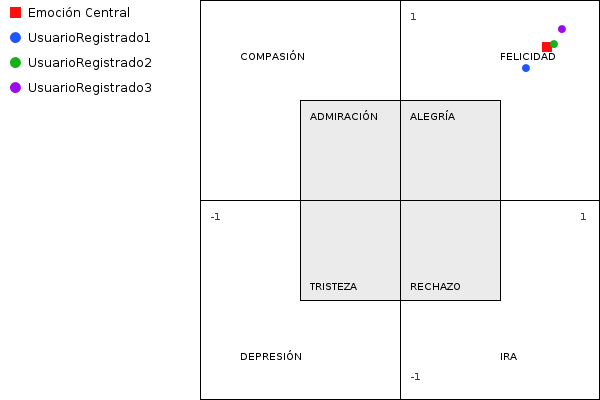
\includegraphics[width=11cm]{ilustraciones/resultados/caso1escenario1-emocioncentral.png}
\end{ilustracion}

\begin{ilustracion}[fuente=\yo, etiqueta=dispersion-emocional-final-caso1escenario1, titulo={Evolución de la Dispersión Emocional ($\sigma(Ag)$), Caso de Estudio 1 Escenario 1}]
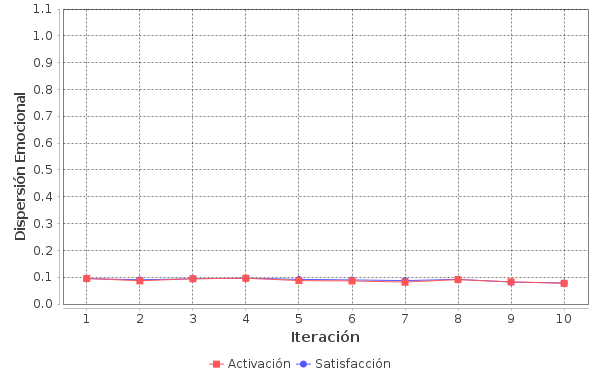
\includegraphics[width=11cm]{ilustraciones/resultados/caso1escenario1-dispersionemocional.png}
\end{ilustracion}

\clearpage
\newpage

\begin{sidewaysfigure}

\begin{cuadro}[etiqueta=resultadoscaso1escenario1, titulo={Evolución de la Emoción Social del Grupo de Agentes ($Ag$), Caso de Estudio 1 Escenario 1}, letra=\tiny]{c|l|l|c|c|l|l|c|c|l|c|c|c|c}
\toprule
\multirow{2}{*}{\textbf{Iteración}} & \multicolumn{6}{c|}{\textbf{Agentes}} &  \multicolumn{3}{c|}{\textbf{$EC(Ag)$}} & \multicolumn{2}{c|}{\textbf{$m(Ag)$}} & \multicolumn{2}{c}{\textbf{$\sigma(Ag)$}} \\ \cline{2-14}
& Nombre & Estímulo & A & S & Emoción & Comportamiento & A & S & Emoción & A & S & A & S \\
\midrule[1pt]
\multirow{3}{*}{0} & UsuarioRegistrado1 & & 0.1 & 0.1 & Alegría & Imitativo & \multirow{3}{*}{0.2} & \multirow{3}{*}{0.2} & \multirow{3}{*}{Alegría} & \multirow{3}{*}{0.1} & \multirow{3}{*}{0.1} & \multirow{3}{*}{0.082} & \multirow{3}{*}{0.082}  \\\cline{2-7}
& UsuarioRegistrado2 & & 0.2 & 0.2 & Alegría & Imitativo & & & & & & & \\ \cline{2-7}
& UsuarioRegistrado3 & & 0.3 & 0.3 & Alegría & Imitativo & & & & & & & \\ \midrule[1pt]
\multirow{3}{*}{1} & UsuarioRegistrado1 & Artículo Nuevo & 0.15 & 0.15 & Alegría & Imitativo & \multirow{3}{*}{0.253} & \multirow{3}{*}{0.257} & \multirow{3}{*}{Alegría} & \multirow{3}{*}{0.127} & \multirow{3}{*}{0.123} & \multirow{3}{*}{0.095} & \multirow{3}{*}{0.095}  \\\cline{2-7}
& UsuarioRegistrado2 & Nueva Edición & 0.23 & 0.24 & Alegría & Imitativo & & & & & & & \\ \cline{2-7}
& UsuarioRegistrado3 & Artículo Sobresaliente & 0.38 & 0.38 & Alegría & Imitativo & & & & & & & \\ \midrule[1pt]
\multirow{3}{*}{2} & UsuarioRegistrado1 & Artículo Nuevo & 0.2 & 0.2 & Alegría & Imitativo & \multirow{3}{*}{0.297} & \multirow{3}{*}{0.303} & \multirow{3}{*}{Alegría} & \multirow{3}{*}{0.113} & \multirow{3}{*}{0.117} & \multirow{3}{*}{0.087} & \multirow{3}{*}{0.09}  \\\cline{2-7}
& UsuarioRegistrado2 & Artículo Nuevo & 0.28 & 0.29 & Alegría & Imitativo & & & & & & & \\ \cline{2-7}
& UsuarioRegistrado3 & Nueva Edición & 0.41 & 0.42 & Alegría & Imitativo & & & & & & & \\ \midrule[1pt]
\multirow{3}{*}{3} & UsuarioRegistrado1 & Nueva Edición & 0.23 & 0.24 & Alegría & Imitativo & \multirow{3}{*}{0.34} & \multirow{3}{*}{0.35} & \multirow{3}{*}{Alegría} & \multirow{3}{*}{0.12} & \multirow{3}{*}{0.12} & \multirow{3}{*}{0.094} & \multirow{3}{*}{0.094}  \\\cline{2-7}
& UsuarioRegistrado2 & Artículo Nuevo & 0.33 & 0.34 & Alegría & Imitativo & & & & & & & \\ \cline{2-7}
& UsuarioRegistrado3 & Artículo Nuevo & 0.46 & 0.47 & Alegría & Imitativo & & & & & & & \\ \midrule[1pt]
\multirow{3}{*}{4} & UsuarioRegistrado1 & Artículo Sobresaliente & 0.31 & 0.32 & Alegría & Imitativo & \multirow{3}{*}{0.41} & \multirow{3}{*}{0.42} & \multirow{3}{*}{Alegría} & \multirow{3}{*}{0.13} & \multirow{3}{*}{0.13} & \multirow{3}{*}{0.096} & \multirow{3}{*}{0.096}  \\\cline{2-7}
& UsuarioRegistrado2 & Artículo Nuevo & 0.38 & 0.39 & Alegría & Imitativo & & & & & & & \\ \cline{2-7}
& UsuarioRegistrado3 & Artículo Sobresaliente & 0.54 & 0.55 & Felicidad & Imitativo & & & & & & & \\ \midrule[1pt]
\multirow{3}{*}{5} & UsuarioRegistrado1 & Artículo Nuevo & 0.36 & 0.37 & Alegría & Imitativo & \multirow{3}{*}{0.453} & \multirow{3}{*}{0.467} & \multirow{3}{*}{Alegría} & \multirow{3}{*}{0.117} & \multirow{3}{*}{0.123} & \multirow{3}{*}{0.087} & \multirow{3}{*}{0.092}  \\\cline{2-7}
& UsuarioRegistrado2 & Artículo Nuevo & 0.43 & 0.44 & Alegría & Imitativo & & & & & & & \\ \cline{2-7}
& UsuarioRegistrado3 & Nueva Edición & 0.57 & 0.59 & Felicidad & Imitativo & & & & & & & \\ \midrule[1pt]
\multirow{3}{*}{6} & UsuarioRegistrado1 & Nueva Edición & 0.39 & 0.41 & Alegría & Imitativo & \multirow{3}{*}{0.5} & \multirow{3}{*}{0.52} & \multirow{3}{*}{Felicidad} & \multirow{3}{*}{0.11} & \multirow{3}{*}{0.11} & \multirow{3}{*}{0.086} & \multirow{3}{*}{0.09}  \\\cline{2-7}
& UsuarioRegistrado2 & Artículo Sobresaliente & 0.51 & 0.52 & Felicidad & Imitativo & & & & & & & \\ \cline{2-7}
& UsuarioRegistrado3 & Nueva Edición & 0.6 & 0.63 & Felicidad & Imitativo & & & & & & & \\ \midrule[1pt]
\multirow{3}{*}{7} & UsuarioRegistrado1 & Artículo Nuevo & 0.44 & 0.46 & Alegría & Imitativo & \multirow{3}{*}{0.553} & \multirow{3}{*}{0.577} & \multirow{3}{*}{Felicidad} & \multirow{3}{*}{0.113} & \multirow{3}{*}{0.117} & \multirow{3}{*}{0.082} & \multirow{3}{*}{0.087}  \\\cline{2-7}
& UsuarioRegistrado2 & Artículo Sobresaliente & 0.59 & 0.6 & Felicidad & Imitativo & & & & & & & \\ \cline{2-7}
& UsuarioRegistrado3 & Nueva Edición & 0.63 & 0.67 & Felicidad & Imitativo & & & & & & & \\ \midrule[1pt]
\multirow{3}{*}{8} & UsuarioRegistrado1 & Nueva Edición & 0.47 & 0.5 & Alegría & Imitativo & \multirow{3}{*}{0.597} & \multirow{3}{*}{0.623} & \multirow{3}{*}{Felicidad} & \multirow{3}{*}{0.127} & \multirow{3}{*}{0.123} & \multirow{3}{*}{0.091} & \multirow{3}{*}{0.092}  \\\cline{2-7}
& UsuarioRegistrado2 & Artículo Nuevo & 0.64 & 0.65 & Felicidad & Imitativo & & & & & & & \\ \cline{2-7}
& UsuarioRegistrado3 & Artículo Nuevo & 0.68 & 0.72 & Felicidad & Imitativo & & & & & & & \\ \midrule[1pt]
\multirow{3}{*}{9} & UsuarioRegistrado1 & Artículo Sobresaliente & 0.55 & 0.58 & Felicidad & Imitativo & \multirow{3}{*}{0.667} & \multirow{3}{*}{0.693} & \multirow{3}{*}{Felicidad} & \multirow{3}{*}{0.117} & \multirow{3}{*}{0.113} & \multirow{3}{*}{0.083} & \multirow{3}{*}{0.082}  \\\cline{2-7}
& UsuarioRegistrado2 & Artículo Sobresaliente & 0.72 & 0.73 & Felicidad & Imitativo & & & & & & & \\ \cline{2-7}
& UsuarioRegistrado3 & Artículo Nuevo & 0.73 & 0.77 & Felicidad & Imitativo & & & & & & & \\ \midrule[1pt]
\multirow{3}{*}{10} & UsuarioRegistrado1 & Artículo Sobresaliente & 0.63 & 0.66 & Felicidad & Imitativo & \multirow{3}{*}{0.737} & \multirow{3}{*}{0.763} & \multirow{3}{*}{Felicidad} & \multirow{3}{*}{0.107} & \multirow{3}{*}{0.103} & \multirow{3}{*}{0.077} & \multirow{3}{*}{0.078}  \\\cline{2-7}
& UsuarioRegistrado2 & Artículo Nuevo & 0.77 & 0.78 & Felicidad & Imitativo & & & & & & & \\ \cline{2-7}
& UsuarioRegistrado3 & Artículo Sobresaliente & 0.81 & 0.85 & Felicidad & Imitativo & & & & & & & \\ \midrule[1pt]
\fuentecuadro{14}{\yo}
\end{cuadro}

\end{sidewaysfigure}

\clearpage
\newpage

\subseccion{Escenario 2: Alta Dispersión Emocional y Bajo Número de Agentes}

En este escenario, se supone un grupo con 3 usuarios registrados, el primero de ellos
solo recibe estímulos que favorecen la emociones positivas, ya que, incrementan la reputación del mismo,
el segundo usuario contribuye a Wikipedia recibiendo diferentes estímulos
que propician emociones tanto positivas como negativas, y el último propone
y desarrolla contenido, pero recibe rechazo por el aporte realizado (estímulos
que favorecen emociones negativas) \refpcuadro{estimulos-propuestos}.
De acuerdo al modelo afectivo de MASOES, estos agentes exhibirían diferentes emociones,
ya que, son expuestos a estímulos que contribuyen a la generación de emociones positivas y negativas,
además, según la definición de emoción social propuesta en este trabajo,
el grupo de agentes presentaría una dispersión emocional elevada.

Al igual que el escenario anterior, se presenta una tabla \refpcuadro{resultadoscaso1escenario2}
que muestra la evolución y el resultado final de la $ES(Ag)$.
En esta simulación, se obtuvo como resultado una $EC(Ag)$ igual a: $(-0.07, -0.05)$
que corresponde a la emoción Tristeza \refpilustracion{emocion-central-final-caso1escenario2}.
Con respecto a la $\sigma(Ag)$, se obtuvieron valores alejados de cero,
tanto para la activación como para la satisfacción: $(0.49, 0.523)$ \refpilustracion{dispersion-emocional-final-caso1escenario2},
así como la $m(Ag)$: $(0.61, 0.65)$. De estos resultados se puede interpretar,
que el grupo de agentes en cuestión exhibe emociones muy heterogéneas, y que
existen estados emocionales muy alejados de la emoción central.
Es importante mencionar en la interpretación, que la $EC(Ag)$
representa de una mejor manera al grupo de agentes a medida que la $\sigma(Ag)$ es más cercana a cero.
Ciertamente, el objetivo de la $EC(Ag)$ es dar una idea de la tendencia de
la emoción que exhibe el grupo de agentes, pero para este caso
aunque la $EC(Ag)$ es Tristeza, solo un agente expresa dicha emoción,
y se debe a que el grupo tiene
una dispersión emocional alejada de cero.

\begin{ilustracion}[fuente=\yo, etiqueta=emocion-central-final-caso1escenario2, titulo={Emoción Central Final, Caso de Estudio 1 Escenario 2}]
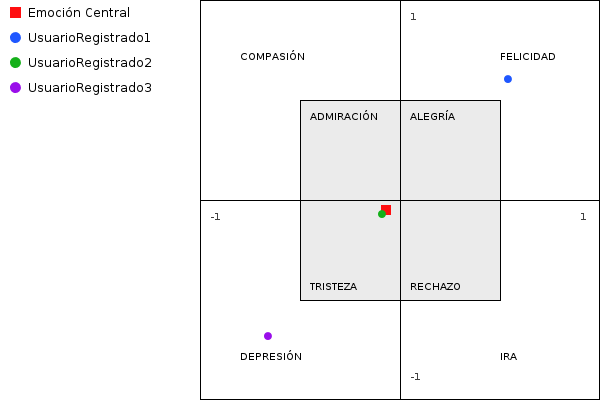
\includegraphics[width=11cm]{ilustraciones/resultados/caso1escenario2-emocioncentral.png}
\end{ilustracion}

\begin{ilustracion}[fuente=\yo, etiqueta=dispersion-emocional-final-caso1escenario2, titulo={Evolución de la Dispersión Emocional ($\sigma(Ag)$), Caso de Estudio 1 Escenario 2}]
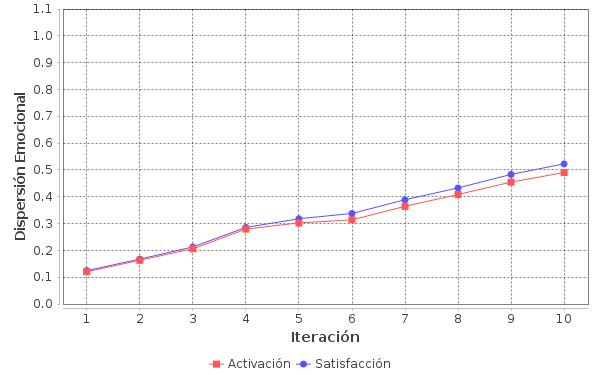
\includegraphics[width=11cm]{ilustraciones/resultados/caso1escenario2-dispersionemocional.png}
\end{ilustracion}

\clearpage
\newpage

\begin{sidewaysfigure}

\begin{cuadro}[etiqueta=resultadoscaso1escenario2, titulo={Evolución de la Emoción Social del Grupo de Agentes ($Ag$), Caso de Estudio 1 Escenario 2}, letra=\tiny]{c|l|l|c|c|l|l|c|c|l|c|c|c|c}
\toprule
\multirow{2}{*}{\textbf{Iteración}} & \multicolumn{6}{c|}{\textbf{Agentes}} &  \multicolumn{3}{c|}{\textbf{$EC(Ag)$}} & \multicolumn{2}{c|}{\textbf{$m(Ag)$}} & \multicolumn{2}{c}{\textbf{$\sigma(Ag)$}} \\ \cline{2-14}
& Nombre & Estímulo & A & S & Emoción & Comportamiento & A & S & Emoción & A & S & A & S \\
\midrule[1pt]
\multirow{3}{*}{0} & UsuarioRegistrado1 & & 0.1 & 0.1 & Alegría & Imitativo & \multirow{3}{*}{0} & \multirow{3}{*}{0} & \multirow{3}{*}{Admiración} & \multirow{3}{*}{0.1} & \multirow{3}{*}{0.1} & \multirow{3}{*}{0.082} & \multirow{3}{*}{0.082}  \\\cline{2-7}
& UsuarioRegistrado2 & & 0 & 0 & Admiración & Imitativo & & & & & & & \\ \cline{2-7}
& UsuarioRegistrado3 & & -0.1 & -0.1 & Tristeza & Cognitivo & & & & & & & \\ \midrule[1pt]
\multirow{3}{*}{1} & UsuarioRegistrado1 & Nueva Edición & 0.13 & 0.14 & Alegría & Imitativo & \multirow{3}{*}{-0.03} & \multirow{3}{*}{-0.027} & \multirow{3}{*}{Tristeza} & \multirow{3}{*}{0.16} & \multirow{3}{*}{0.167} & \multirow{3}{*}{0.12} & \multirow{3}{*}{0.125}  \\\cline{2-7}
& UsuarioRegistrado2 & Artículo Borrado & -0.06 & -0.06 & Tristeza & Cognitivo & & & & & & & \\ \cline{2-7}
& UsuarioRegistrado3 & Artículo Borrado & -0.16 & -0.16 & Tristeza & Cognitivo & & & & & & & \\ \midrule[1pt]
\multirow{3}{*}{2} & UsuarioRegistrado1 & Artículo Nuevo & 0.18 & 0.19 & Alegría & Imitativo & \multirow{3}{*}{-0.017} & \multirow{3}{*}{-0.013} & \multirow{3}{*}{Tristeza} & \multirow{3}{*}{0.203} & \multirow{3}{*}{0.207} & \multirow{3}{*}{0.163} & \multirow{3}{*}{0.167}  \\\cline{2-7}
& UsuarioRegistrado2 & Artículo Nuevo & -0.01 & -0.01 & Tristeza & Cognitivo & & & & & & & \\ \cline{2-7}
& UsuarioRegistrado3 & Artículo Borrado & -0.22 & -0.22 & Tristeza & Cognitivo & & & & & & & \\ \midrule[1pt]
\multirow{3}{*}{3} & UsuarioRegistrado1 & Nueva Edición & 0.21 & 0.23 & Alegría & Imitativo & \multirow{3}{*}{0} & \multirow{3}{*}{0.007} & \multirow{3}{*}{Admiración} & \multirow{3}{*}{0.28} & \multirow{3}{*}{0.287} & \multirow{3}{*}{0.206} & \multirow{3}{*}{0.213}  \\\cline{2-7}
& UsuarioRegistrado2 & Artículo Sobresaliente & 0.07 & 0.07 & Alegría & Imitativo & & & & & & & \\ \cline{2-7}
& UsuarioRegistrado3 & Artículo Borrado & -0.28 & -0.28 & Tristeza & Cognitivo & & & & & & & \\ \midrule[1pt]
\multirow{3}{*}{4} & UsuarioRegistrado1 & Artículo Sobresaliente & 0.29 & 0.31 & Alegría & Imitativo & \multirow{3}{*}{0.027} & \multirow{3}{*}{0.033} & \multirow{3}{*}{Alegría} & \multirow{3}{*}{0.387} & \multirow{3}{*}{0.393} & \multirow{3}{*}{0.279} & \multirow{3}{*}{0.286}  \\\cline{2-7}
& UsuarioRegistrado2 & Artículo Sobresaliente & 0.15 & 0.15 & Alegría & Imitativo & & & & & & & \\ \cline{2-7}
& UsuarioRegistrado3 & Guerra de Ediciones & -0.36 & -0.36 & Tristeza & Cognitivo & & & & & & & \\ \midrule[1pt]
\multirow{3}{*}{5} & UsuarioRegistrado1 & Nueva Edición & 0.32 & 0.35 & Alegría & Imitativo & \multirow{3}{*}{0.04} & \multirow{3}{*}{0.05} & \multirow{3}{*}{Alegría} & \multirow{3}{*}{0.42} & \multirow{3}{*}{0.44} & \multirow{3}{*}{0.302} & \multirow{3}{*}{0.318}  \\\cline{2-7}
& UsuarioRegistrado2 & Nueva Edición & 0.18 & 0.19 & Alegría & Imitativo & & & & & & & \\ \cline{2-7}
& UsuarioRegistrado3 & Artículo Modificado & -0.38 & -0.39 & Tristeza & Cognitivo & & & & & & & \\ \midrule[1pt]
\multirow{3}{*}{6} & UsuarioRegistrado1 & Nueva Edición & 0.35 & 0.39 & Alegría & Imitativo & \multirow{3}{*}{0.023} & \multirow{3}{*}{0.033} & \multirow{3}{*}{Alegría} & \multirow{3}{*}{0.423} & \multirow{3}{*}{0.453} & \multirow{3}{*}{0.314} & \multirow{3}{*}{0.338}  \\\cline{2-7}
& UsuarioRegistrado2 & Artículo Borrado & 0.12 & 0.13 & Alegría & Imitativo & & & & & & & \\ \cline{2-7}
& UsuarioRegistrado3 & Artículo Modificado & -0.4 & -0.42 & Tristeza & Cognitivo & & & & & & & \\ \midrule[1pt]
\multirow{3}{*}{7} & UsuarioRegistrado1 & Artículo Sobresaliente & 0.43 & 0.47 & Alegría & Imitativo & \multirow{3}{*}{0.003} & \multirow{3}{*}{0.013} & \multirow{3}{*}{Alegría} & \multirow{3}{*}{0.463} & \multirow{3}{*}{0.493} & \multirow{3}{*}{0.364} & \multirow{3}{*}{0.389}  \\\cline{2-7}
& UsuarioRegistrado2 & Guerra de Ediciones & 0.04 & 0.05 & Alegría & Imitativo & & & & & & & \\ \cline{2-7}
& UsuarioRegistrado3 & Artículo Borrado & -0.46 & -0.48 & Tristeza & Cognitivo & & & & & & & \\ \midrule[1pt]
\multirow{3}{*}{8} & UsuarioRegistrado1 & Artículo Nuevo & 0.48 & 0.52 & Felicidad & Imitativo & \multirow{3}{*}{-0.027} & \multirow{3}{*}{-0.017} & \multirow{3}{*}{Tristeza} & \multirow{3}{*}{0.507} & \multirow{3}{*}{0.537} & \multirow{3}{*}{0.408} & \multirow{3}{*}{0.433}  \\\cline{2-7}
& UsuarioRegistrado2 & Guerra de Ediciones & -0.04 & -0.03 & Tristeza & Cognitivo & & & & & & & \\ \cline{2-7}
& UsuarioRegistrado3 & Artículo Borrado & -0.52 & -0.54 & Depresión & Reactivo & & & & & & & \\ \midrule[1pt]
\multirow{3}{*}{9} & UsuarioRegistrado1 & Nueva Edición & 0.51 & 0.56 & Felicidad & Imitativo & \multirow{3}{*}{-0.07} & \multirow{3}{*}{-0.057} & \multirow{3}{*}{Tristeza} & \multirow{3}{*}{0.58} & \multirow{3}{*}{0.617} & \multirow{3}{*}{0.455} & \multirow{3}{*}{0.483}  \\\cline{2-7}
& UsuarioRegistrado2 & Guerra de Ediciones & -0.12 & -0.11 & Tristeza & Cognitivo & & & & & & & \\ \cline{2-7}
& UsuarioRegistrado3 & Guerra de Ediciones & -0.6 & -0.62 & Depresión & Reactivo & & & & & & & \\ \midrule[1pt]
\multirow{3}{*}{10} & UsuarioRegistrado1 & Nueva Edición & 0.54 & 0.6 & Felicidad & Imitativo & \multirow{3}{*}{-0.07} & \multirow{3}{*}{-0.05} & \multirow{3}{*}{Tristeza} & \multirow{3}{*}{0.61} & \multirow{3}{*}{0.65} & \multirow{3}{*}{0.49} & \multirow{3}{*}{0.523}  \\\cline{2-7}
& UsuarioRegistrado2 & Nueva Edición & -0.09 & -0.07 & Tristeza & Cognitivo & & & & & & & \\ \cline{2-7}
& UsuarioRegistrado3 & Artículo Borrado & -0.66 & -0.68 & Depresión & Reactivo & & & & & & & \\ \midrule[1pt]
\fuentecuadro{14}{\yo}
\end{cuadro}

\end{sidewaysfigure}

\clearpage
\newpage

\subseccion{Escenario 3: Baja Dispersión Emocional y Alto Número de Agentes}

Como MASOES es una arquitectura que permite modelar
sistemas emergentes y auto-organizados con alta densidad de agentes,
se plantea este escenario con el objetivo de verificar el cálculo de la $ES(Ag)$, con alto
número de agentes y baja dispersión emocional.
Se configura una simulación con 50 agentes emocionales y 20 iteraciones,
e inicializan los estados emocionales de manera aleatoria en todo el modelo afectivo,
y no para una sola emoción. En cada iteracion se envían intencionalmente para todos los agentes, estímulos
que favorecen una emoción positiva (incrementan la reputación de los wikipedistas).

En la \refcuadro{emocion-social-caso1escenario3}, se presentan la $ES(Ag)$ inicial y final.
Con respecto a los valores iniciales, se observa que
la $EC(Ag)$ exhibe Alegría, con $m(Ag)$ y $\sigma(Ag)$ iguales a: (0.98, 1.119) y
(0.59, 0.624), respectivamente. De esto se puede interpretar, que
el grupo de agentes tiene una alta dispersión emocional (emociones muy heterogéneas) al iniciar la simulación,
la \refilustracion{emocion-central-inicial-caso1escenario3} muestra una representación
gráfica del estado inicial.
Los valores finales obtenidos muestran
una disminución en la dispersión emocional,
se obtuvo una $EC(Ag)$ igual a Felicidad: (0.764, 0.829) \refpilustracion{emocion-central-final-caso1escenario3},
con $m(Ag)$ igual a: (0.697, 0.755) y una $\sigma(Ag)$
de (0.305, 0.293).
Es importante resaltar, que para realizar una interpretación adecuada de la $ES(Ag)$,
es necesario analizar sus componentes ($EC(Ag)$,  $m(Ag)$ y $\sigma(Ag)$), sobre todo la $\sigma(Ag)$.
Para este caso, aunque la $EC(Ag)$ inicial fue Alegría, pocos agentes mostraban dicha emoción,
pero al finalizar la simulación, la mayoría de los agentes si exhibían Felicidad
tal como la $EC(Ag)$, y se debe a una disminución en la $\sigma(Ag)$, en otras palabras,
los estados emocionales de los agentes se aproximaron,
esto puede ser apreciado en \refilustracion{dispersion-emocional-final-caso1escenario3}.
Los valores resultantes develan la importancia que representa la $\sigma(Ag)$ para
la propuesta de $ES(Ag)$ presentada en este trabajo.

Otro aspecto interesante en la simulación, es que en los estados emocionales finales
algunos de los agentes tuvieron una activación o satisfacción igual a 1, esto se debe a que solo
recibieron estímulos que propician emociones positivas y sus estados emocionales llegaron al límite
del modelo afectivo.

\begin{cuadro}[etiqueta=emocion-social-caso1escenario3, titulo={Valor Inicial y Final de la Emoción Social del Grupo de Agentes ($Ag$), Caso 1 Escenario 3}]{llll}
\toprule
 &  $EC(Ag)$ & $m(Ag)$ & $\sigma(Ag)$ \\
\midrule
Inicial & (0.001, 0.125) Alegría & (0.98, 1.119) & (0.59, 0.624) \\
Final & (0.764, 0.829) Felicidad & (0.697, 0.755) & (0.305, 0.293) \\
\bottomrule
\fuentecuadro{4}{\yo}
\end{cuadro}

\begin{ilustracion}[fuente=\yo, etiqueta=emocion-central-inicial-caso1escenario3, titulo={Emoción Central Inicial, Caso de Estudio 1 Escenario 3}]
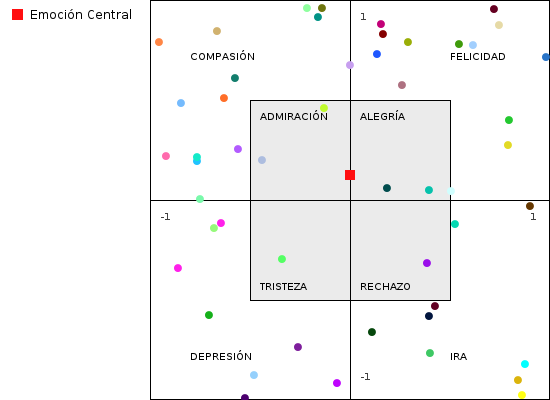
\includegraphics[width=10cm]{ilustraciones/resultados/caso1escenario3-emocioncentral-inicial.png}
\end{ilustracion}

\begin{ilustracion}[fuente=\yo, etiqueta=emocion-central-final-caso1escenario3, titulo={Emoción Central Final, Caso de Estudio 1 Escenario 3}]
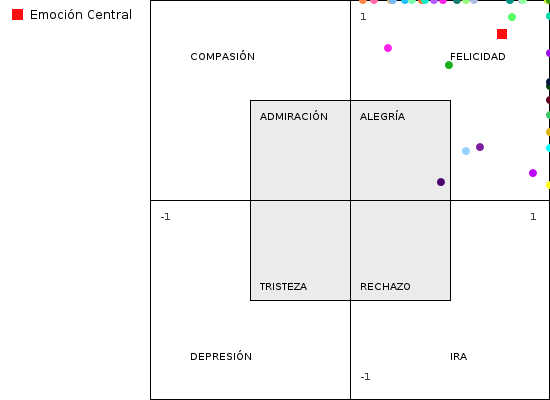
\includegraphics[width=10cm]{ilustraciones/resultados/caso1escenario3-emocioncentral-final.png}
\end{ilustracion}

\begin{ilustracion}[fuente=\yo, etiqueta=dispersion-emocional-final-caso1escenario3, titulo={Evolución de la Dispersión Emocional ($\sigma(Ag)$), Caso de Estudio 1 Escenario 3}]
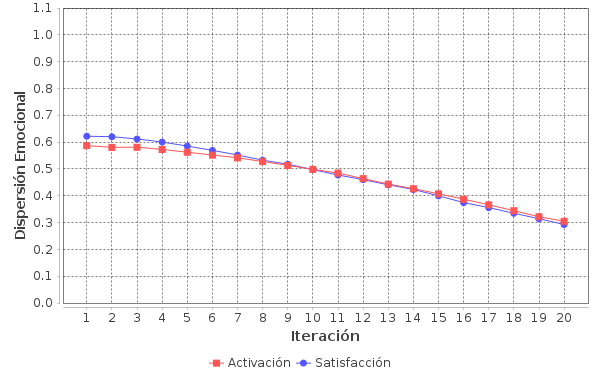
\includegraphics[width=11cm]{ilustraciones/resultados/caso1escenario3-dispersionemocional.png}
\end{ilustracion}

\clearpage
\newpage

\subseccion{Escenario 4: Alta Dispersión Emocional y Alto Número de Agentes}

Siguiendo la misma idea que el escenario anterior,
para este se configura una simulación con 50 agentes emocionales y 20 iteraciones,
e inicializan los estados emocionales de manera aleatoria en todo el modelo afectivo,
no obstante, se envían estímulos que incrementan la reputación al 50\%
de los wikipedistas (25 agentes) y estímulos que decrementan la reputación al otro 50\%,
con el objetivo de verificar la generación de la $ES(Ag)$ en un grupo con alto
número de agentes y alta $\sigma(Ag)$.

Los resultados obtenidos \refpcuadro{emocion-social-caso1escenario4},
muestran que la $EC(Ag)$ se modificó ligeramente pasando de (-0.138, -0.142)
a (-0.076, -0.067), manteniéndose en Tristeza,
lo interesante en este escenario es el resultado
obtenido en la $\sigma(Ag)$, como se muestra en la \refilustracion{dispersion-emocional-final-caso1escenario4},
se incrementó tanto para la activación como para la satisfacción, debido
a que los estados emocionales se fueron distanciando (muy heterogéneos), aun así
la $EC(Ag)$ se mantuvo en Tristeza. Una de las conclusiones para esto,
es que el número de agentes no influye en el resultado de la $EC(Ag)$,
más la $\sigma(Ag)$ si es un factor importante a tomar en cuenta a la hora
de hacer una interpretación. Además, se puede observar en la
\refilustracion{emocion-central-inicial-caso1escenario4} como los estados emocionales de los
agentes se distribuyen por todo el modelo afectivo al iniciar la simulación
y al finalizarla los agentes se
concentraron en los cuadrantes 1 (Alegría y Felicidad)
y 4 (Tristeza y Depresión) como se muestra en la \refilustracion{emocion-central-final-caso1escenario4},
es decir, dos grupos. Esto abre una oportunidad de investigación futura, en la que se puedan generar más de una
$ES(Ag)$ dependiendo del número de agrupaciones de estados emocionales exhibidos.

De igual manera que el escenario anterior,
para algunos de los agentes se obtuvo una activación o satisfacción igual a 1 o -1 en el resultado final,
esto se debe a que solo recibieron un tipo de estímulos, que incrementa o decrementa la reputación
y los estados emocionales llegaron al valor mínimo o máximo permitido según el modelo afectivo de MASOES.

\begin{cuadro}[etiqueta=emocion-social-caso1escenario4, titulo={Valor Inicial y Final de la Emoción Social del Grupo de Agentes ($Ag$), Caso 1 Escenario 4}]{llll}
\toprule
 &  $EC(Ag)$ & $m(Ag)$ & $\sigma(Ag)$ \\
\midrule
Inicial & (-0.138, -0.142) Tristeza & (1.051, 1.115) & (0.598, 0.652) \\
Final & (-0.076, -0.067) Tristeza & (1.076, 1.067) & (0.831, 0.743) \\
\bottomrule
\fuentecuadro{4}{\yo}
\end{cuadro}

\begin{ilustracion}[fuente=\yo, etiqueta=emocion-central-inicial-caso1escenario4, titulo={Emoción Central Inicial, Caso de Estudio 1 Escenario 4}]
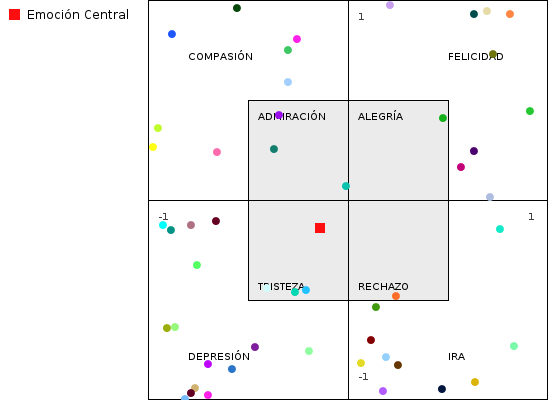
\includegraphics[width=10cm]{ilustraciones/resultados/caso1escenario4-emocioncentral-inicial.png}
\end{ilustracion}

\begin{ilustracion}[fuente=\yo, etiqueta=emocion-central-final-caso1escenario4, titulo={Emoción Central Final, Caso de Estudio 1 Escenario 4}]
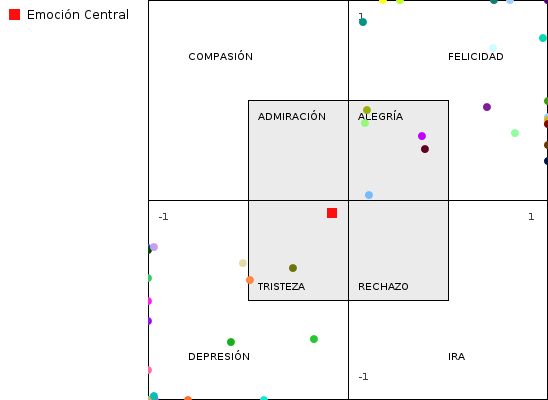
\includegraphics[width=10cm]{ilustraciones/resultados/caso1escenario4-emocioncentral-final.png}
\end{ilustracion}

\begin{ilustracion}[fuente=\yo, etiqueta=dispersion-emocional-final-caso1escenario4, titulo={Evolución de la Dispersión Emocional ($\sigma(Ag)$), Caso de Estudio 1 Escenario 4}]
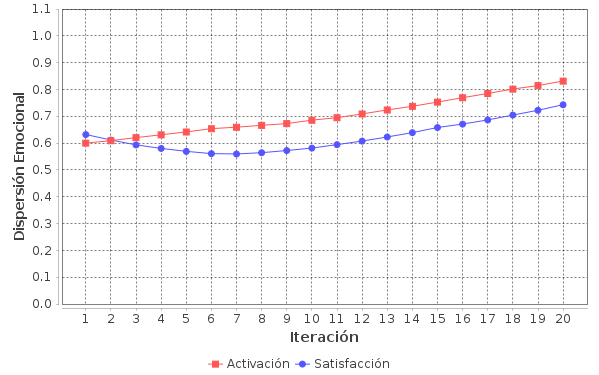
\includegraphics[width=11cm]{ilustraciones/resultados/caso1escenario4-dispersionemocional.png}
\end{ilustracion}

\clearpage
\newpage

\seccion{Caso de Estudio 2: Emociones a Nivel Individual}

El objetivo de este caso de estudio es verificar que el modelo afectivo propuesto en
MASOES a nivel de implementación, genere correctamente emociones positivas y negativas
individualmente en los agentes emocionales. A través de dos escenarios atómicos,
se generarán emociones y se comparará los resultados con los obtenidos
a nivel de diseño en \cite{perozo2012}.
Para esto se realiza una simulación en ambos escenarios con un agente de tipo Usuario Registrado
y 20 iteraciones.

\subseccion{Escenario 1: Grado de Satisfacción Alto y Activación Alto, Medio y Bajo}

Para este escenario, un colaborador propone y desarrolla un contenido, recibiendo
un incremento de reputación por la calidad del aporte realizado. Este usuario
podría experimentar un alto grado de satisfacción y activación, que se
traduciría en emociones positivas individuales, lo que conllevaría a un
comportamiento imitativo para tratar de repetir esta experiencia,
de acuerdo al modelo afectivo de MASOES. Esto se debe a que según el espacio afectivo definido
\refpilustracion{modelo-afectivo}, al permanecer alto el grado de satisfacción
del agente y variar el grado de activación, se siguen promoviendo las emociones
positivas, bien sean individuales o sociales (cuadrantes 1 y 2 del espacio
afectivo bidimensional). Por lo dicho anteriormente, se seleccionan
solo estímulos que incrementan la reputación del agente \refpcuadro{estimulos-propuestos}.
Se inicializa el agente con un satisfacción igual a 1, ya que, se tiene como objetivo observar la evolución del estado emocional
siendo afectado únicamente por la activación y se asigna una activación baja de -0.6,
estos valores corresponden a la emoción Compasión.

Sobre los resultados, en la \refilustracion{emociones-individuales-escenerio1-estado-emocional-colaborador1} se observa que
aunque la satisfacción se mantiene constante, la activación se incrementó.
A su vez,
en la \refilustracion{emociones-individuales-escenario1-modificacion-de-emociones}, se refleja que
la emoción asociada al estado actual del agente fue modificándose a medida que la activación iba
en incremento, pasando de compasión a felicidad y la \refilustracion{emociones-individuales-escenario1-modificacion-de-comportamiento},
muestra que el agente se mantuvo con un comportamiento imitativo.

Los resultados obtenidos permiten verificar que
la implementación cumple con lo elaborado a nivel de diseño \citep{perozo2012}, al permanecer alto el grado de satisfacción del
agente y variar el grado de activación, se siguen promoviendo las emociones positivas,
bien sean individuales o sociales. En
otras palabras, a pesar de variar el grado de activación y producir emociones menos o
más intensas, el agente mantuvo su comportamiento imitativo.

\begin{ilustracion}[fuente=\yo, etiqueta=emociones-individuales-escenerio1-estado-emocional-colaborador1, titulo={Variación del Estado Emocional del Agente, Caso de Estudio 2 Escenario 1}]
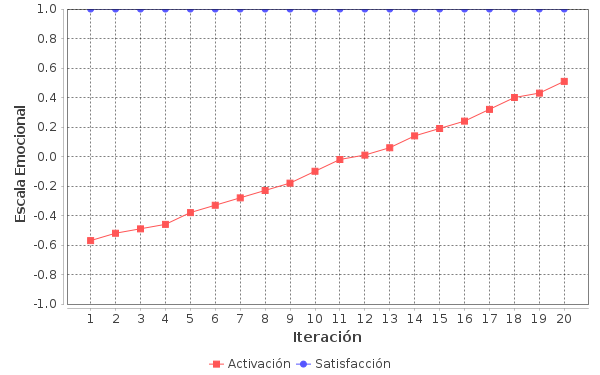
\includegraphics[width=11cm]{ilustraciones/resultados/caso2escenerio1-estado-emocional-colaborador1.png}
\end{ilustracion}

\begin{ilustracion}[fuente=\yo, etiqueta=emociones-individuales-escenario1-modificacion-de-emociones, titulo={Variación de la Emoción Exhibida por el Agente, Caso de Estudio 2 Escenario 1}]
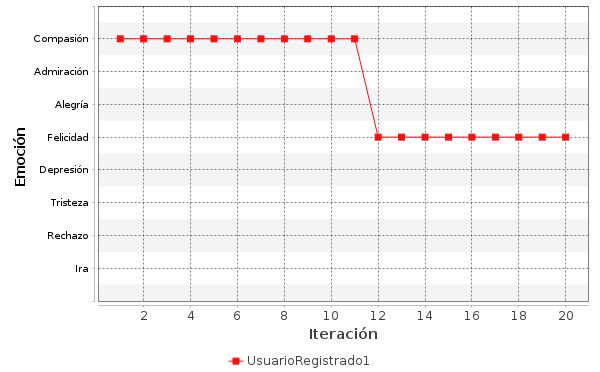
\includegraphics[width=11cm]{ilustraciones/resultados/caso2escenerio1-modificacion-de-emociones.png}
\end{ilustracion}

\begin{ilustracion}[fuente=\yo, etiqueta=emociones-individuales-escenario1-modificacion-de-comportamiento, titulo={Variación del Comportamiento Exhibido por el Agente, Caso de Estudio 2 Escenario 1}]
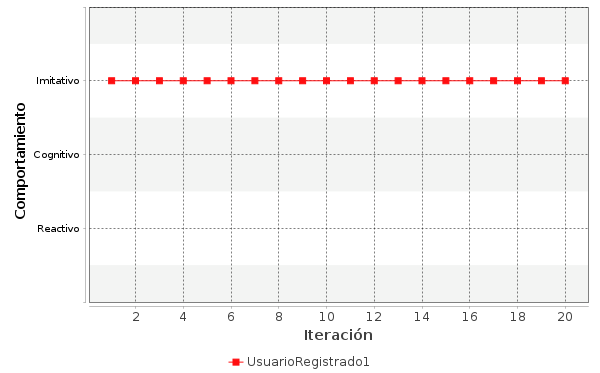
\includegraphics[width=11cm]{ilustraciones/resultados/caso2escenerio1-modificacion-de-comportamiento.png}
\end{ilustracion}

\clearpage
\newpage

\subseccion{Escenario 2: Grado de Satisfacción y Activación Medio y Bajo}

A diferencia de lo anterior, en este escenario un usuario registrado propone y desarrolla un contenido,
el cual amerita modificaciones por la comunidad, recibiendo
un decremento de reputación por el aporte realizado. Este usuario
podría experimentar disminución del grado de satisfacción y activación,
provocándole emociones negativas y activando un comportamiento
cognitivo o reactivo.
Se seleccionan
solo estímulos que decrementan la reputación del agente \refpcuadro{estimulos-propuestos}.
El agente es inicializado en la emoción Alegría con una activación de 0.5
y satisfacción 0.3.

Con respecto a los resultados, en la \refilustracion{emociones-individuales-escenerio2-estado-emocional-colaborador1}, se puede observar
la disminución en la activación y satisfacción del estado emocional del agente.
Los resultados reflejan que el agente varió su emoción pasando de alegría a rechazo, tristeza y depresión \refpilustracion{emociones-individuales-escenario2-modificacion-de-emociones}.
Así mismo, la \refilustracion{emociones-individuales-escenario2-modificacion-de-comportamiento}
muestra la variación de comportamientos del agente, el cual inició con comportamiento imitativo
pero fue actualizado a un comportamiento de tipo cognitivo y posteriormente uno reactivo.
Estos valores concuerdan con los escenarios 2 y 3 expuestos
en \cite{perozo2012}, la disminución de reputación en el agente afectará tanto la activación
como la satisfacción de su estado emocional,
provocándole emociones negativas y activando un comportamiento
reactivo o cognitivo.

\begin{ilustracion}[fuente=\yo, etiqueta=emociones-individuales-escenerio2-estado-emocional-colaborador1, titulo={Variación del Estado Emocional del Agente, Caso de Estudio 2 Escenario 2}]
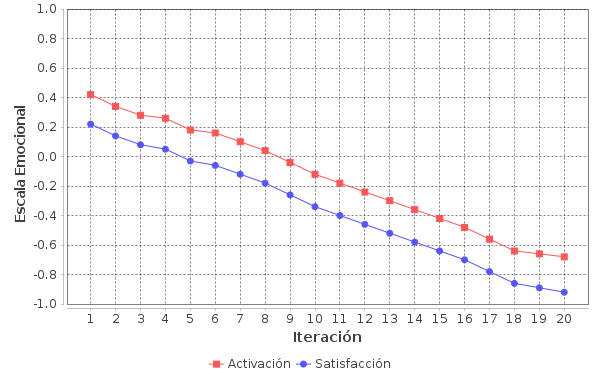
\includegraphics[width=11cm]{ilustraciones/resultados/caso2escenerio2-estado-emocional-colaborador1.png}
\end{ilustracion}

\begin{ilustracion}[fuente=\yo, etiqueta=emociones-individuales-escenario2-modificacion-de-emociones, titulo={Variación de la Emoción Exhibida por el Agente, Caso de Estudio 2 Escenario 2}]
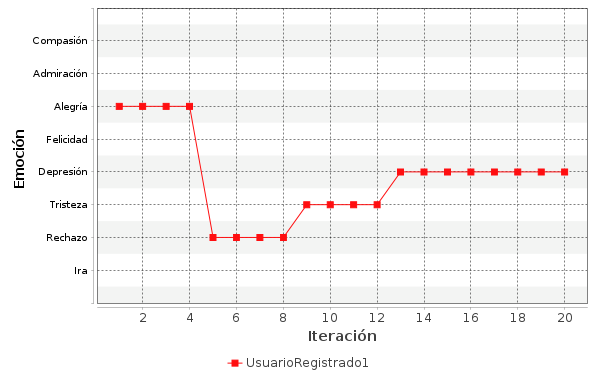
\includegraphics[width=11cm]{ilustraciones/resultados/caso2escenerio2-modificacion-de-emociones.png}
\end{ilustracion}

\begin{ilustracion}[fuente=\yo, etiqueta=emociones-individuales-escenario2-modificacion-de-comportamiento, titulo={Variación del Comportamiento Exhibido por el Agente, Caso de Estudio 2 Escenario 2}]
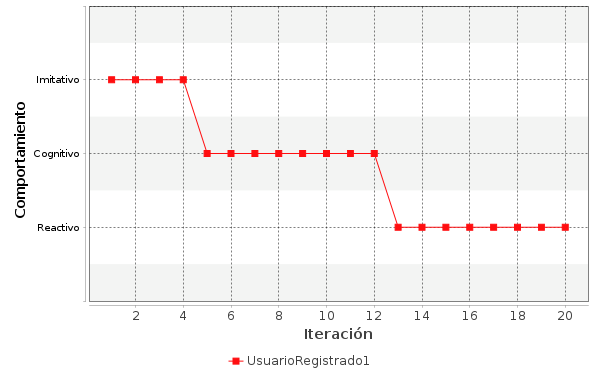
\includegraphics[width=11cm]{ilustraciones/resultados/caso2escenerio2-modificacion-de-comportamiento.png}
\end{ilustracion}
